%%%%%%%%%%%%%%%%%%%%%%%%%%%%%%%%%%%%%%%%%
% Masters/Doctoral Thesis 
% LaTeX Template
% Version 2.5 (27/8/17)
%
% This template was downloaded from:
% http://www.LaTeXTemplates.com
%
% Version 2.x major modifications by:
% Vel (vel@latextemplates.com)
%
% This template is based on a template by:
% Steve Gunn (http://users.ecs.soton.ac.uk/srg/softwaretools/document/templates/)
% Sunil Patel (http://www.sunilpatel.co.uk/thesis-template/)
%
% Template license:
% CC BY-NC-SA 3.0 (http://creativecommons.org/licenses/by-nc-sa/3.0/)
%
%%%%%%%%%%%%%%%%%%%%%%%%%%%%%%%%%%%%%%%%%

%----------------------------------------------------------------------------------------
%	PACKAGES AND OTHER DOCUMENT CONFIGURATIONS
%----------------------------------------------------------------------------------------

\documentclass[
11pt, % The default document font size, options: 10pt, 11pt, 12pt
oneside, % Two side (alternating margins) for binding by default, uncomment to switch to one side
english, % ngerman for German
singlespacing, % Single line spacing, alternatives: onehalfspacing or doublespacing
%draft, % Uncomment to enable draft mode (no pictures, no links, overfull hboxes indicated)
%nolistspacing, % If the document is onehalfspacing or doublespacing, uncomment this to set spacing in lists to single
%liststotoc, % Uncomment to add the list of figures/tables/etc to the table of contents
%toctotoc, % Uncomment to add the main table of contents to the table of contents
%parskip, % Uncomment to add space between paragraphs
%nohyperref, % Uncomment to not load the hyperref package
headsepline, % Uncomment to get a line under the header
%chapterinoneline, % Uncomment to place the chapter title next to the number on one line
%consistentlayout, % Uncomment to change the layout of the declaration, abstract and acknowledgements pages to match the default layout
table,
]{MastersDoctoralThesis} % The class file specifying the document structure

\usepackage[utf8]{inputenc} % Required for inputting international characters
\usepackage[T1]{fontenc} % Output font encoding for international characters

\usepackage{mathpazo} % Use the Palatino font by default
\usepackage{float}

\usepackage[backend=bibtex,style=authoryear,natbib=true,doi=false]{biblatex} % Use the bibtex backend with the authoryear citation style (which resembles APA)

\addbibresource{references.bib} % The filename of the bibliography

\usepackage[autostyle=true]{csquotes} % Required to generate language-dependent quotes in the bibliography
\usepackage{eurosym}

%----------------------------------------------------------------------------------------
%	MARGIN SETTINGS
%----------------------------------------------------------------------------------------

\geometry{
	paper=a4paper, % Change to letterpaper for US letter
	inner=2.5cm, % Inner margin
	outer=3.8cm, % Outer margin
	bindingoffset=.5cm, % Binding offset
	top=1.5cm, % Top margin
	bottom=1.5cm, % Bottom margin
	%showframe, % Uncomment to show how the type block is set on the page
}

%----------------------------------------------------------------------------------------
%	THESIS INFORMATION
%----------------------------------------------------------------------------------------

\thesistitle{Analysis of the SVM-RFE algorithm for feature selection} % Your thesis title, this is used in the title and abstract, print it elsewhere with \ttitle
\supervisor{Luis A. \textsc{Belanche}} % Your supervisor's name, this is used in the title page, print it elsewhere with \supname
\examiner{} % Your examiner's name, this is not currently used anywhere in the template, print it elsewhere with \examname
\degree{Bachelor Degree in Informatics Engineering} % Your degree name, this is used in the title page and abstract, print it elsewhere with \degreename
\author{Robert \textsc{Planas}} % Your name, this is used in the title page and abstract, print it elsewhere with \authorname
\addresses{} % Your address, this is not currently used anywhere in the template, print it elsewhere with \addressname

\subject{Computing} % Your subject area, this is not currently used anywhere in the template, print it elsewhere with \subjectname
\keywords{} % Keywords for your thesis, this is not currently used anywhere in the template, print it elsewhere with \keywordnames
\university{\href{http://www.upc.edu}{Universitat Politècnica de Catalunya}} % Your university's name and URL, this is used in the title page and abstract, print it elsewhere with \univname
\department{ \_ } % Your department's name and URL, this is used in the title page and abstract, print it elsewhere with \deptname
\group{ \_ } % Your research group's name and URL, this is used in the title page, print it elsewhere with \groupname
\faculty{Facultat d'informàtica de Barcelona} % Your faculty's name and URL, this is used in the title page and abstract, print it elsewhere with \facname

\AtBeginDocument{
\hypersetup{pdftitle=\ttitle} % Set the PDF's title to your title
\hypersetup{pdfauthor=\authorname} % Set the PDF's author to your name
\hypersetup{pdfkeywords=\keywordnames} % Set the PDF's keywords to your keywords
}

\begin{document}

\frontmatter % Use roman page numbering style (i, ii, iii, iv...) for the pre-content pages

\pagestyle{plain} % Default to the plain heading style until the thesis style is called for the body content

%----------------------------------------------------------------------------------------
%	TITLE PAGE
%----------------------------------------------------------------------------------------

\begin{titlepage}
\begin{center}

\vspace*{.06\textheight}
{\scshape\LARGE \univname\par}\vspace{0.5cm} % University name
\textsc{\Large \facname}\\[1.5cm] % Facultry name
\Large{GEP \ — \  Deliverable 2}\\[0.2cm] % Thesis type
\small{\emph{GEP tutor:} Andujar Larios}\\[0.5cm]

\HRule \\[0.4cm] % Horizontal line
{\huge \bfseries \ttitle\par}\vspace{0.4cm} % Thesis title
\HRule \\[1.5cm] % Horizontal line
 
\begin{minipage}[t]{0.4\textwidth}
\begin{flushleft} \large
\emph{Author:}\\
\href{http://www.hubbit86.com}{\authorname} % Author name - remove the \href bracket to remove the link
\end{flushleft}
\end{minipage}
\begin{minipage}[t]{0.4\textwidth}
\begin{flushright} \large
\emph{Director:} \\
\href{https://www.cs.upc.edu/~belanche/}{\supname} % Supervisor name - remove the \href bracket to remove the link  
\end{flushright}
\end{minipage}\\[4cm]

\vfill

\large \degreename\\ % Speciality name
\large Specialization:  Computing\\[0.5cm] % Speciality name

\vfill

% \large \textit{A thesis submitted in fulfillment of the requirements\\ for the degree of \degreename}\\[0.3cm] % University requirement text
% \textit{in the}\\[0.4cm]
% \groupname\\\deptname\\[2cm] % Research group name and department name

\includegraphics{logo.pdf} % University/department logo - uncomment to place it

\vfill

{\large \today}\\[4cm] % Date

\vfill
\end{center}
\end{titlepage}



%----------------------------------------------------------------------------------------
%	THESIS CONTENT - CHAPTERS
%----------------------------------------------------------------------------------------

\newcommand{\tabhead}[1]{\textbf{#1}}

\mainmatter % Begin numeric (1,2,3...) page numbering

\pagestyle{thesis} % Return the page headers back to the "thesis" style
\tableofcontents
\chapter{Non-linear Kernels} % Main chapter title

\label{Chapter1} % For referencing the chapter elsewhere, use \ref{Chapter1} 
\label{eq:ch4.grankingcoeff}

%----------------------------------------------------------------------------------------

This modification intends to apply the required modifications in the calculation of the ranking criteria so that non-linear kernels can be used in the SVM.

\section{Description and reasoning}
\label{sec:stopCond.desc}

When a problem is not linearly separable, we know that a hard-margin SVM will not be able to correctly place a decision boundary. In this case a soft-margin SVM may be used, but it only works to some extent and if the underlying distribution is near linearly separable. If it is not the case, much better results can be achieved by using non-linear kernels.

To use this method within SVM-RFE we must first be able to compute the ranking coefficient from a non-linear kernel. In contrast with the linear kernel case, where the ranking coefficient can be simplified to $(w_i)^2$, for non-linear kernels, however, since it is a more general case, no simplification can be performed. Instead, we use the general ranking coefficient for SVM (Equation \ref{eq:ch4.grankingcoeff}), which we restate here:
\begin{align*}
    DJ(i) = (1/2)(\boldsymbol{\alpha}^\T \vb{H} \boldsymbol{\alpha} - \boldsymbol{\alpha}^\T \vb{H}(-i) \boldsymbol{\alpha})
\end{align*}

Note that the \emph{hessian} matrix $\vb{H_{i,j}} = y_iy_jk(\vb{x_i}, \vb{x_j})$ needs be computed each iteration (since the dimension of $\vb{x_i}$ and $\vb{x_j}$ will change), and also for each feature removed in each iteration. This is slow, however various optimizations may exist, as discussed in Section [ref.].

\section{Pseudocode formalization}

\textbf{Definitions:}

\begin{itemize}
    \item $X_0 = [\vt{x_0}, \vt{x_1}, \dotsc, \vt{x_k}]^T$ list of observations.
    \item $\vt{y} = [y_1, y_2, \dotsc, y_k]^T$ list of labels.
\end{itemize}

\begin{algorithm}[H]
    \DontPrintSemicolon
      \KwInput{$t, k$ \tcp*{$t$ = step, $k$ = kernel function}}
      \KwOutput{$\vt{r}$}
      \KwData{$X_0,\vt{y}$}
      $\vt{s} = [1,2, \dotsc, n]$ \tcp*{subset of surviving features}
      $\vt{r} = []$ \tcp*{feature ranked list}
      \While{$|\vt{s}| > 0$}
        {
            \tcc*[h]{Restrict training examples to good feature indices}\\
            $X=X_0(:,\vt{s})$\VS

            \tcc*[h]{Precompute hessian matrix}\\
            $\vb{H_{i,j}} = y_iy_jk(\vb{x_i}, \vb{x_j}) \qquad \text{for all} \qquad \vb{x_i}, \vb{x_j} \in X$\VS

            \tcc*[h]{Train the classifier}\\
            $\vt{\alpha} = \texttt{SVM-train(} X, y, k \texttt{)}$\VS

            \tcc*[h]{Compute the ranking criteria}\\
            $\vt{c} = [c_1, c_2, \dots, c_{|\vt{s}|}]$ \\
            \For{$c_l \in \vt{c}$}{
                \tcc*[h]{Compute new hessian with the feature $l$ removed}\\
                $\vb{H_{i,j}}(-l) = y_iy_jk(\vb{x_i}, \vb{x_j}) \qquad \text{for all} \qquad \vb{x_i}, \vb{x_j} \in X(-l)$\VS
    
                \tcc*[h]{Calculate ranking coefficient}\\
                $c_l = (1/2)(\boldsymbol{\alpha}^\T \vb{H} \boldsymbol{\alpha} - \boldsymbol{\alpha}^\T \vb{H}(-l) \boldsymbol{\alpha})$
            }\VS

            \tcc*[h]{Find the $t$ features with the smallest ranking criterion}\\
            $\vt{f} = \texttt{argsort}(\vt{c})(\ :t)$\VS

            \tcc*[h]{Iterate over the feature subset}\\
            \For{$f_i \in \vt{f}$}{
                \tcc*[h]{Update the feature ranking list}\\
                $\vt{r} = [\vt{s}(f_i), ...\vt{r}]$\VS
    
                \tcc*[h]{Eliminate the feature selected}\\
                $\vt{s} = [...\vt{s}(1:f_i - 1), ...\vt{s}(f_i + 1:|\vt{s}|)]$
            }
        }
    \caption{SVM-RFE with Stop Condition}
    \label{alg:svmrfe-stopcond}
\end{algorithm}

\section{Results}


% Chapter 1

\chapter{Project Planning} % Main chapter title
\label{Chapter2} % For referencing the chapter elsewhere, use \ref{Chapter1} 

\newcommand{\tabhead}[1]{\textbf{#1}}

%----------------------------------------------------------------------------------------

This thesis is worth 15 ECTS credits, each of which with an estimate cost of 25 to 30 hours. Therefore, the total time allocated for this project, as indicated by the faculty, is of 375 to 450 hours. This time is to be distributed in 100 days, from 03/08/21 to 06/15/21, with an estimated work of 4 to 5 hours a day. The date of the oral defense is planned for the first week of July, this sets the deadline to be on the 06/18/21.

An extra 3 ECTS credits are to be used for project managment, this is roughly 80 hours, which makes the total time estimate for the whole project (Theisis + Project Managment) to be at best 450 hours and at worse 540 hours. In order to make a proper plannification, we have defined the estimated cost to be at 500 hours.

\section{Task definition}

In this section it is presented all the tasks that will be carried out along the project. For each, a description, duration and a list of dependencies with other tasks are given.

Project management is a mandatory group of such tasks, albeit not very useful, considering that: One, this project is done by a single individual, with assistance from a project director; And two, this is a research project, which makes planning of specific tasks difficult, since it is the results from the research that drive the next steps to be done.  

\begin{itemize}
    \item \textbf{Context and scope:} We have to indicate the general objective(s) of the project, contextualize it and justify the reason for selecting this subject area.
    \item \textbf{Project planning:} This will help us not lose focus while we're working on the project.
    \item \textbf{Budget and sustainability:} For this specific project, this is irrelevant. The budget required is negligible and already defrayed; and the impact, beyond trivial matters, is likely zero and otherwise unknown. 
    \item \textbf{Final project definition:} Review the work done in the project management tasks.
    \item \textbf{Meetings:} Online meetings are scheduled once every two weeks with the tutor of the project. Discussion of the status and next tasks to do will be done.
\end{itemize}

This project is research focused. Therefore, before starting the practical tasks research on the various topics needs to be done. This will involve collecting and analyzing previous studies that tried new methods and extensions to the SVM-RFE algorithm. We will also have to document ourselves in the SVM and feature selection areas, as well as the algorithms and the statistical theory used in the studies. Some basic understanding of bioinformatics may also be required considering the use case of most if these studies.

\begin{itemize}
    \item \textbf{Research} previous work on the literature on extensions of the algorithm and create a short \textbf{report} with the findings.
    \item Write the algorithm formalization in pseudocode.
    \item Define the expected advantages or disadvantages of this method over the base SVM-RFE.
    \item Compute the space and time complexities.
\end{itemize}

Once the initial research is done the algorithm must be codified and tested. This group is composed of the following tasks:

\begin{itemize}
    \item \textbf{Program the base SVM-RFE algorithm.} For this we will use a library for the SVM. For the RFE part, since we need to be able to extend the algorithm, we will program it from scratch.
    \item \textbf{Program the extensions of the SVM-RFE algorithm} based on the research done and the pseudocode.
    \item \textbf{Test the new extensions with artificial data.} This requires creating models and testing their performance with artificial data sets.
    \item \textbf{Obtain data sets with real data.} Multiple papers refer to publically available data-sets, we could use those and compare our results.
    \item \textbf{Test the new extensions with real data.} This requires creating models and testing their performance with real data sets.
    \item \textbf{Analyze the results} obtained in the experiments and draw conclusions. A report will be made for reference during the final documentation.
\end{itemize}


Once finished, the final documenting phase will begin. Firstly, we will collect all the information obtained in the experimental and analysis part, which will be available in the form of the reports that we've done along the tasks. Afterwards, we can start writing the documentation of the project. This will include a fairly extensive review on concepts related to SVM, statistics, feature selection and RFE. Finally, we will have to prepare for the oral defense of the project.

\begin{table}
\centering
\begin{tabular}{l l l l}
\toprule
\tabhead{ID} & \tabhead{Description} & \tabhead{Hours} & \tabhead{Dependencies} \\
\midrule
\rowcolor{gray!10} T1 & Project Managment & 80 &  \\
T1.1 & Context and Scope & 20 & T2.1  \\
T1.2 & Project planning & 10 & \\
T1.3 & Budget  and  sustainability & 10 & T1.2 \\
T1.4 & Final project definition & 20 & T1.1, T1.2, T1.3  \\
T1.5 & Meetings & 20 &  \\
\rowcolor{gray!10} T2 & Theoretical Part & 160 &  \\
T2.1 & Research & 90 &  \\
T2.2 & Formalize & 20 & T2.1  \\
T2.3 & Analyze & 50 & T2.2 \\
\rowcolor{gray!10} T3 & Practical Part & 160 &  \\
T3.1 & Program the base SVM-RFE algorithm & 10 & T2.1  \\
T3.2 & Program the extensions & 50 & T2.1, T3.1  \\
T3.3 & Test with artificial data & 20 & T3.2  \\
T3.4 & Test with real data & 30 & T3.2  \\
T3.5 & Analyze  the  results & 50 & T3.3, T3.4 \\
\rowcolor{gray!10} T4 & Documentation & 100 &  \\
T4.1 & Writte the documentation & 80 & T2, T3  \\
T4.2 & Prepare the thesis defense & 20 & T4.1  \\
\bottomrule\\
\end{tabular}
\caption{Summary and time estimates of the tasks.}
\label{tab:tasks}
\end{table}

\begin{figure}[H]
    \centering
    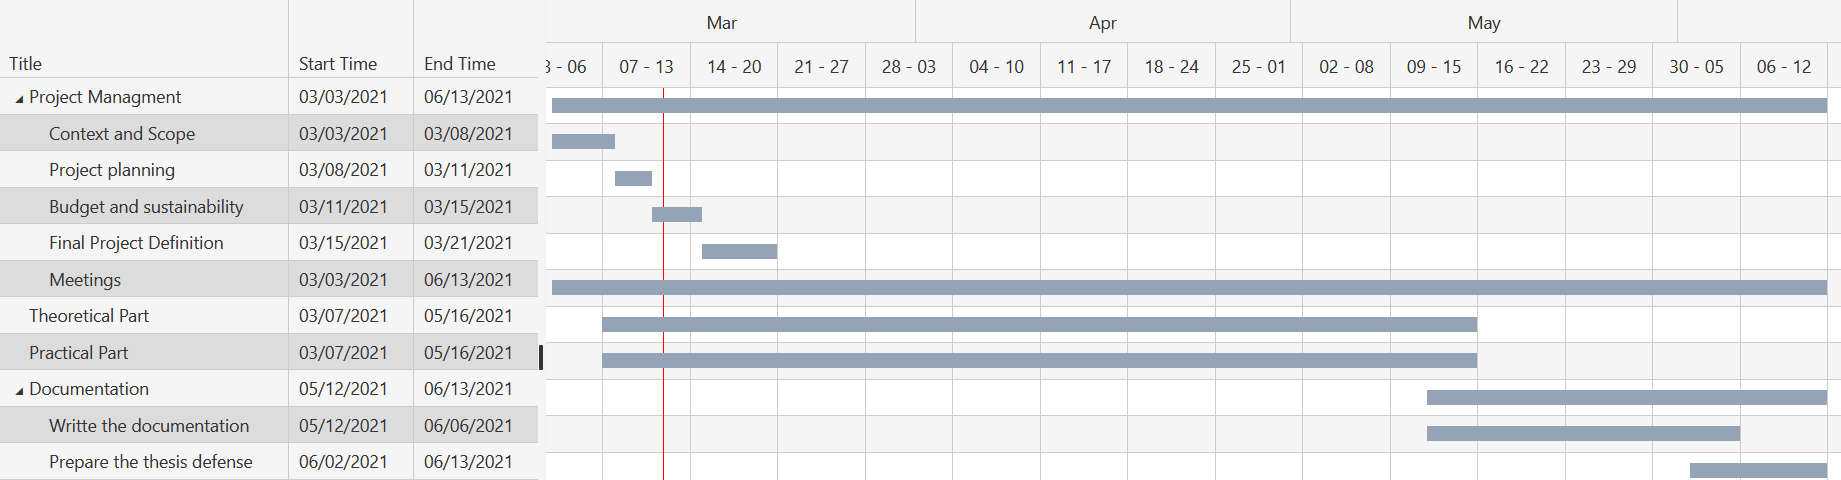
\includegraphics[scale=0.35]{gantt.png}
    \caption{A summary of the tasks represented with a gantt chart. Notice that all the theoretical and practical tasks are done in parallel.}
    \label{fig:gantt}
\end{figure}

\section{Resources}

Our project needs resources to carry out its correct development. These resources have been divided in 4 different groups: human, hardware, software and material resources.

\subsection{Human resources}

There are three human resources that are directly involved in this project.

\begin{itemize}
    \item \textbf{The researcher:} He is responsible for the development of the project, that is, he will have to plan, analyze, program, experiment and document the project.
    \item \textbf{The director/tutor:} He is responsible for leading and guiding the researcher for the correct development of the project.
    \item \textbf{The GEP tutor:} He is in charge of reviewing the project management tasks done in the initial stage of the project.
\end{itemize}

\subsection{Hardware Resources}

The most essential resource needed is a computer connected to the internet. In this project a personal computer will be used. Its specializations are 16 GB of RAM and a CPU \emph{AMD Ryzen 7 4800HS}, with a base speed of 2.9 GHz and 8 cores. Hardware required for a connection to the internet (a router, an access point, etc) is also taken into account.

\subsection{Software Resources}

For project management tasks \texttt{Google Calendar} will be used. A number of other Google products such as \texttt{Google Mail}, \texttt{Google Drive} or \texttt{Google Meet} will also be used as tools required for communication with the director or storing of information.

The documentation will be written in \LaTeX, a document preparation system often used in academia. It has the advantage to integrate well with version control systems. A \LaTeX \ template named "\texttt{Masters/Doctoral Thesis}" will be used to facil\-itate the type\-setting and styling of the document. This template was made by Vel and Johannes Böttcher and licensed under \texttt{LPPL 1.3}, based on previous work from Steve R. Gun and Sunil Patel and used with minor modifications. The original is available at \url{http://www.latextemplates.com/}. The document will be written with the \texttt{Microsft Visual Studio Code} editor, using the \texttt{LaTeX Workshop} extension, and it will be compiled with the \texttt{MiKTex} distribuition installed on a \texttt{Linux} machine run\-ning virtualized within a \texttt{WSL} container on top of the actual operating system, a \texttt{Microsoft Windows 10}. For browsing the internet the latest available version of the \texttt{Firefox} web browser will be used, and references to papers will be kept with the \texttt{Zotero} reference manager.

For the practical part, the programming language of choice will be \texttt{Python3}. This is currently one of the programming languages with better popularity in machine learning and related applications. Various libraries and software packages will be used for different tasks. For parsing datasets the \texttt{pandas} library will be used. For data visualization the \texttt{mathplotlib} library will be used. Also, a general tool-set designed for machine learning, the library \texttt{sklearn}, will be used. Finally, code will be documented in-place during its development with the \texttt{Jupyter Notebook} software.

Other libraries and software packages could also be used if the need arises. 

\section{Risk Management}

The potential risks and obstacles have already been introduced in section \ref{sec:risk}. In this section we will focus on a contingency plan to mitigate the risks.

\begin{itemize}
    \item \textbf{Deadline of the project:} The flexibility of the Kanban methodology should help us modify our schedule and working hours if required. If it becomes apparent that the deadline will not be meet, an extension of the deadline can be requested.
    \item \textbf{Bugs on some libraries:} Alternative libraries can be used. If no alternative is found, because most of the used libraries are open source, a \emph{bugfix} could be implemented.
    \item \textbf{Insufficient computational power:} This can be mitigated by using a small sample of the data-set. This though, can induce a small performance reduction, and thus make the results not comparable with each other. 
    \item \textbf{Hardward related issues:} To avoid it data loss, all code and documentation will be routinely uploaded to the cloud in a \texttt{GitHub} repository and \texttt{Google Drive} account.
\end{itemize}




% Chapter 3

\chapter{Budget and Sustainability} % Main chapter title
\label{Chapter3}

In this section a budget estimation will be made. It will include personel costs per task, generic costs and other costs. Moreover, some questions regarding the sustainability aspect of the project will be answered.

\section{Budget}
\label{sec:budget}

\subsection{Costs by role and activity}

In this section we will add the personnel costs to the tasks defined in section \ref{sec:tasks}. For each task a cost will be calculated based on the hourly pay wage per role and the time spend each. Four roles have been defined with their corresponding hourly wage, these are:

\begin{itemize}
    \item The \textbf{project manager} (T1) who is responsible for leading the project direction, planning and correct development.
    \item The \textbf{researcher} (T2), who must perform research in the topic and related ideas, experiment, analyze the results and draw conclusions from them.
    \item The \textbf{programmer} (T3), who must set up the developer environment, code the algorithms in the specified programming language and test them for cor\-rect\-ness.
    \item The \textbf{technical writer} (T4), who is responsible for writting this project doc\-u\-men\-ta\-tion. This includes the reports for each task that requires it and the final thesis.
\end{itemize}

These roles have a clear mapping to the task groups defined in table \ref{tab:tasks}. All roles will be played by the researcher (see section \ref{sec:human_resources}) except the project manager role, which will be played by the researcher, the director and the GEP tutor. For a detailed description of each task cost see table \ref{tab:task_cost}.

Notice that, altough we aligned the project roles with the task groups to simplify our calculations, it is not required to do so. A more complicated scheme where multiple tasks are assigned to a given role is also possible. In such cases we would also have to think about weather the work distribuition is even or not, and assign percentages if it isn't.

\newpage

\begin{table}[h]
    \centering
    \begin{tabular}{l c c c c r}
    \toprule
    \tabhead{Role} & \tabhead{Year (\euro)} & \tabhead{Year +SS (\euro)} & \tabhead{Hour +SS (\euro)} & \tabhead{Task} & \tabhead{Task Cost (\euro)} \\
    \midrule
    Project Manager & 39 000 & 50 700 & 28.7 & T1 & 2 296 \\
    Researcher & 32 000 & 41 600 & 23.5  & T2 & 3 760\\
    Programmer & 26 000 & 33 800 & 19.1  & T3 & 3 065\\
    Technical writer & 22 000 & 28 600 & 16.2 & T4 & 1 260 \\
    \midrule
    \textbf{Total} & & & & & \textbf{10 381} \\
    \bottomrule\\
    \end{tabular}
    \caption{Anual estimated salary for the different project roles  (\cite{noauthor_salarios_2017}). The amount of working hours in a year is defined to be 1764. \emph{+SS indicates “Social Security included”}.}
    \label{tab:task_cost}
\end{table}

\subsection{Generic costs}

\subsubsection*{Amortization}

In this section the amortization costs for the resources purchased in a single payment are calculated. Notice that since all the software used is free and open source, it doesn't contribuite to the cost, thus it is not displayed here. In fact, the only resource that is valid for an amortization analysis is the computer specified in section \ref{sec:hardware_resources}.

The equation we use to compute the amortization cost for each resource is the following:

\begin{equation}
    \text{Amortization (\euro)} = \text{Cost (\euro)} \times \frac{1}{4\text{ years}} \times \frac{1}{100\text{ days}} \times \frac{1}{5\text{ hours}} \times \text{Hours Used}  
\end{equation}

If we apply the amortization equation to the computer, which we purchased for \euro999.95, and assuming 500 hours of usage, its estimated amrotized cost is \euro249.98.

\subsubsection*{Electric cost}

In this section we only calculate a rough estimate. Calculating accurately the cost of electricity involves many variables, and it's outside the scope of this thesis. The average cost of electricity in Spain, in therms of kWh, is \euro0.12. We only count the cost when the hardware is turned on. The following table (\ref{tab:electric_cost}) shows the individual and total cost per item.

\begin{table}[h]
    \centering
    \begin{tabular}{l c c c r}
    \toprule
    \tabhead{Item} & \tabhead{Power (W)} & \tabhead{Time used (h)} & \tabhead{Consumption (kWh)} & \tabhead{Cost (\euro)} \\
    \midrule
    Computer & 180 & 500 & 90 & 10.8 \\
    Router & 10 & 500 & 5 & 0.6 \\
    \midrule
    \textbf{Total} & & & & \textbf{11.4} \\
    \bottomrule
    \end{tabular}
    \caption{Electric cost estimate.}
    \label{tab:electric_cost}
\end{table}

\subsubsection*{Internet cost}

The internet cost in my current location is \euro29.00 per month, this is roughly about \euro0.95 per day (variance is introduced becouse a month length is not constant). The amount of working hours per day is assumed to be 5, thus the total cost the whole project is:

$$
\text{\euro}0.95\text{ /day} \times 100 \text{ days} \times 5/24 \text{ hours} = \text{\euro}19.79
$$

\subsubsection*{Work space}

This project will be developed at my parents home at Figueres, with a rent of \euro400. Since the amount of people living there is 2, the actual cost is \euro200.

\subsubsection*{Total generic costs}

Table \ref{tab:generic_cost} summarizes the total generic costs of this project.

\begin{table}[h]
    \centering
    \begin{tabular}{l r}
    \toprule
    \tabhead{Group} & \tabhead{Cost (\euro)} \\
    \midrule
    Amortization & 249.98 \\
    Electricity & 11.4 \\
    Internet & 19.79 \\
    Rent & 200 \\
    \midrule
    \textbf{Total} & \textbf{481.17} \\
    \bottomrule
    \end{tabular}
    \caption{Total generic cost estimate.}
    \label{tab:generic_cost}
\end{table}

\subsection{Other costs}

\subsubsection*{Contingencies}

Unexcpected problems that were not foreseen may appear during the development of the project, which would take part of our budget. For this reason it as always a good idea to prepare a contingency budget calculated from the budgets we've calculated up to now. We will apply a 10\% contingency margin, that is \euro108.62.

\subsubsection*{Incidental cost}

Unexpected problems that were foreseen and can be mitigated are descrived in section \ref{sec:risk_management}. Some of these mitigations may incur some extra cost. To be able to handle that cost in this section we will calculate a budget based on the previsible problems, their chances of actually ocurring, and the expected cost associated for solving them.

\begin{itemize}
    \item \textbf{Deadline of the project:} If an extension of the deadline is requested, that would require extra hours expend by the researcher. Assuming the extra time required to be 50 hours that would give us a cost of \euro1,175.
    \item \textbf{Bugs on some libraries:} Implementing a \emph{bugfix} we assume would cost arround 20 hours, a task done by the programmer. The estimated cost is \euro382. The risk is small.
    \item \textbf{Insufficient computational power:} If using smaller datasets where not an option, we would abandon the project, since purchasing a new, more powerful, computer or renting a supercomputer is too expensive. The risk is very small.
    \item \textbf{Hardward related issues:} New hardware would be purchased, if possible only the faulty component would be replaced. This would have an estimated cost of about \euro100. The risk is small.
\end{itemize}

The following table summarized the expected cost due to foreseen incidents.

\begin{table}[h]
    \centering
    \begin{tabular}{l r r r}
    \toprule
    \tabhead{Risk} & \tabhead{Expected (\euro)} & \tabhead{Risk (\%)} & \tabhead{Cost (\euro)} \\
    \midrule
    Deadline of the project & 1 175 & 30 & 352.5 \\
    Bugs on some libraries & 382 & 10 & 38.2 \\
    Insufficient computational power & & 5 &  \\
    Hardward related issues & 100 & 10 & 10 \\
    \midrule
    \textbf{Total} & & & \textbf{400.7} \\
    \bottomrule
    \end{tabular}
    \caption{Total incidental cost estimate.}
    \label{tab:incident_cost}
\end{table}

\subsection{Total cost}

The total cost for the project is summarized in table \ref{tab:total_cost}. The cost has been computed as the sum of the justified costs explained in the other sections of the budget plan.

\begin{table}[h]
    \centering
    \begin{tabular}{l r}
    \toprule
    \tabhead{Section} & \tabhead{Cost (\euro)} \\
    \midrule
    Costs by role and activity & 10 381.00 \\
    Generic costs & 481.17 \\
    Other costs & 509.32 \\
    \midrule
    \textbf{Total} & \textbf{11 371.49} \\
    \bottomrule
    \end{tabular}
    \caption{Total cost estimate.}
    \label{tab:total_cost}
\end{table}

\section{Sustainability}

This project does not have a major environmental impact, since it's a re\-search project. Still, some impact, a very small amount, is expected from the electricity consumption and hardware used. This can hardly be reduced, as is required for the development of the project. If the poject succeds at finding improvement to the SVM-RFE al\-go\-rithm, it will reduce computing power requierments for future researches that use it compared to the state-of-the-art solutions. Beocuse this algorithm is used in medical research, a substantial improvement could create a chain reaction that benefits the health of the population in general. This is, however, a very optimistic expectation.

\subsection{Environmental dimension}

\subsubsection*{Have you estimated the environmental impact of undertaking the project?}

This project will not have a major environmental impact. Still, some impact, a very small amount, is present in the form of electricity consumption and the method used by the provider to generte such electricity. Also, the hardware used will eventually contribuite to the technological waste problem, not to mention the environmental cost for their production.

\subsubsection*{Have you considered how to minimise the impact, for example by reusing re\-sources?}

The impact is directly derived from the project requirments and can thus not be reduced easily. A low-cost computer doesn't nescesarly imply a lower impact on the environment or lower electricity consumption. Recycling is of course always an option, but the decision to do so will be taken way after the project has been completed.

\subsubsection*{How is the problem that you wish to address resolved currently (state of the art)? In what ways will your solution environmentally improve exist\-ing solutions?}

This project will use the same resources as those used in state-of-the-art alternatives. Therefore, this solution does not environmentally improve existing solutions. If the project succeeds at funding an improvement to the SVM-RFE agorithm however, it could imply a reduction on computational power required to solve some problems, and thus also a reduction in power consumption.

\subsection{Economic dimension}

\subsubsection*{Have you estimated the cost of undertaking the project (human and material re\-sources)?}

Yes, see section \ref{sec:budget}.

\subsubsection*{How is the problem that you wish to address resolved currently (state of the art)? In what ways will your solution economically improve existing solutions?}

If improvements to the SVM-RFE are found in this project, this will make any re\-search that makes use of less expensive.

\subsection{Social dimension}

\subsubsection*{What do you think undertaking the project has contributed to you personally?}

This is the last step required to finish my degree in computer science. Finalizing this degree will allow me to enter the laboral market and become self-sufficient. Beyond that, it has introduced me to the fields of bioinformatics and data mining, as well as shown the importance of feature analysis and how it can be not just a cleaning prerequisite for a more important problem, but the main dish. 

\subsubsection*{How is the problem that you wish to address resolved currently (state of the art)? In what ways will your solution socially improve (quality of life) existing. Is there a real need for the project?}

Improvements to the SVM-RFE algorithm may or may not be found. Even if found it is still unknown if they will be substantial enough. Moreover, an analysis of the variants of the algorithm will be useful for those who want to use SVM-RFE in the most optimal way.


%----------------------------------------------------------------------------------------
%	BIBLIOGRAPHY
%----------------------------------------------------------------------------------------

\printbibliography[heading=bibintoc]

%----------------------------------------------------------------------------------------

\end{document}  
